\begin{figure}[h]
\begin{center}
	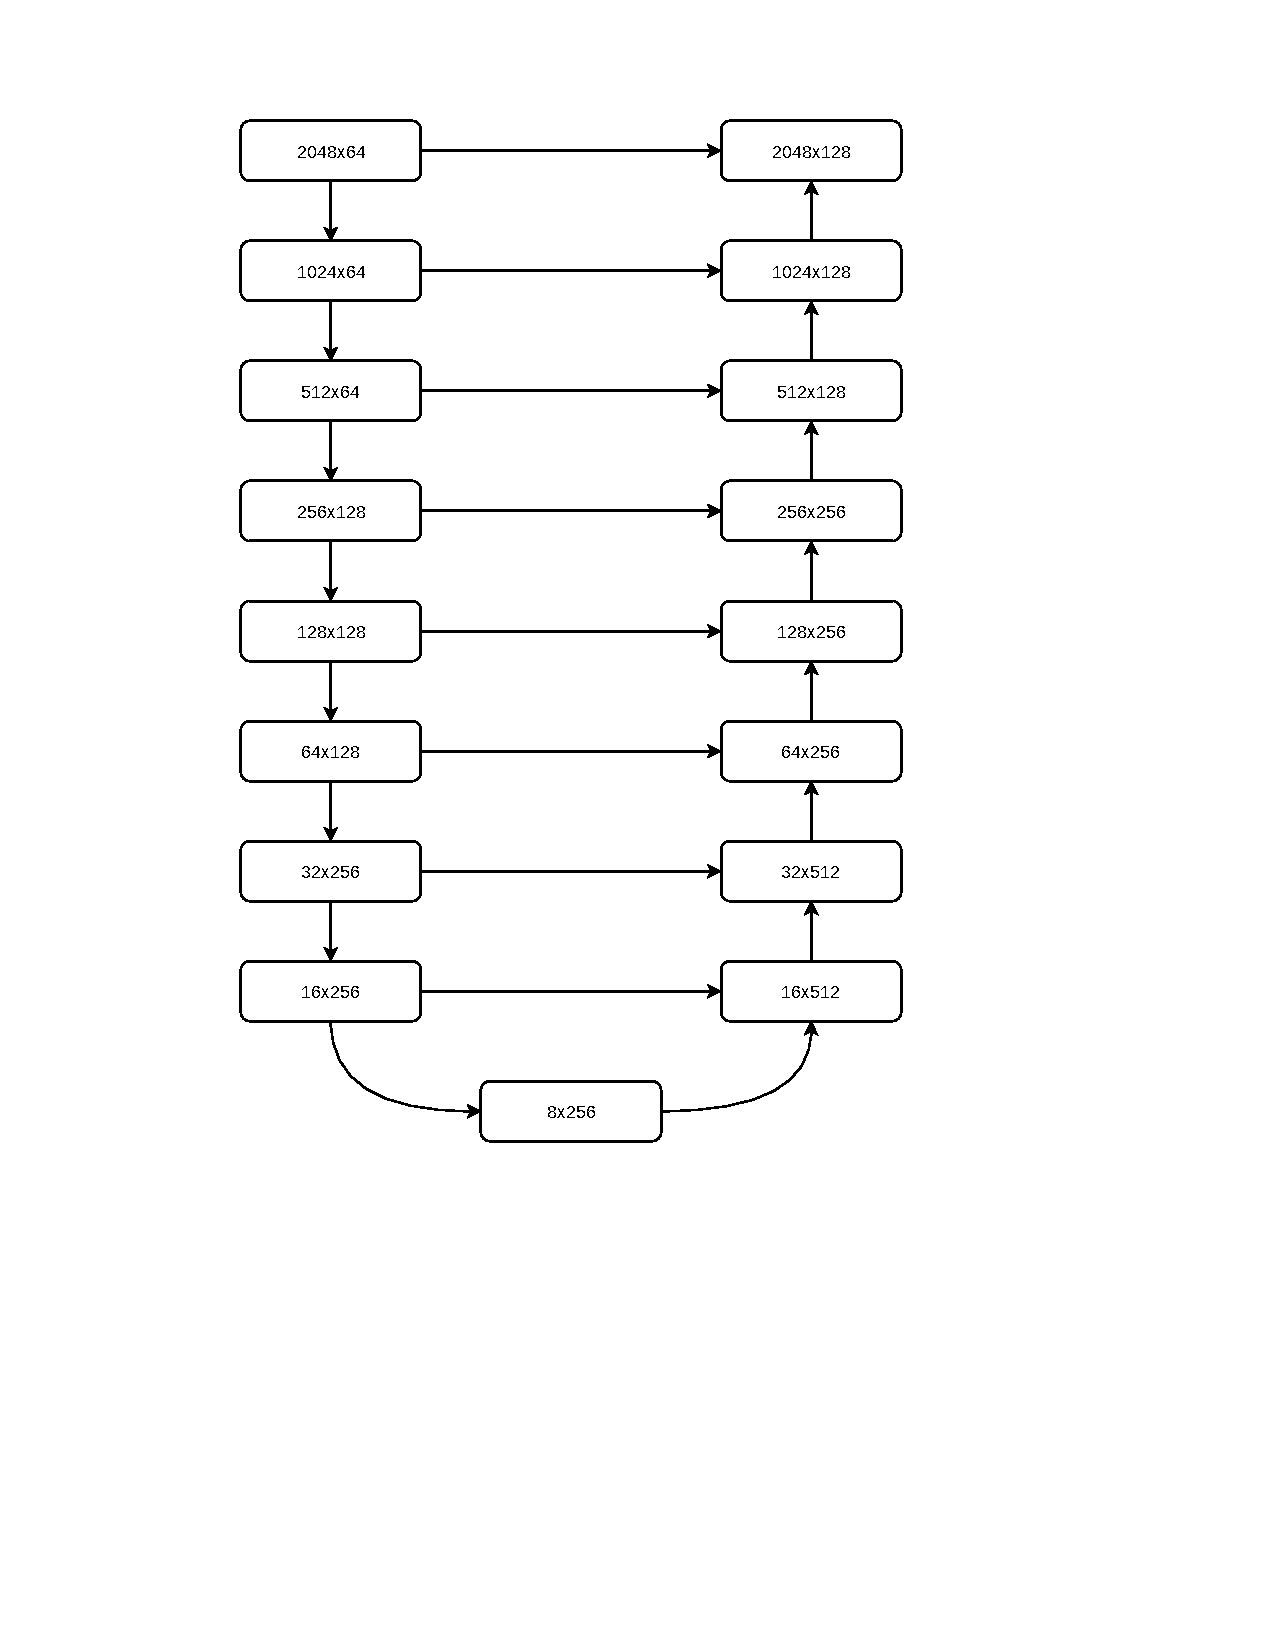
\includegraphics[width=0.5\textwidth]{architecture}
	\caption{Model Architecture}
	\label{fig:architecture}
\end{center}
\end{figure}

\noindent Two networks are trained which are both based on the U-Net architecture originally proposed for speech enhancement/denoising in \cite{pandey_new_2019}.  The reasoning behind using a U-Net architecture is that speech is known to be sparse, and can be represented well with a small amount of data. The information bottleneck of a U-Net architecture should allow the network to distill salient information about the speech, while the pass-through connections allow for the recreation of utterance-specific details. Additionally, the 1-dimensional convolution layers used are known to be useful for frequency analysis, enabling the time-domain network to learn frequency-domain features. The specific layer sizes and the architecture of each block is detailed in figure \ref{fig:architecture}. An \ac{LSTM} is used to filter the latent representation of the speech stored in the bottleneck of the u-net. This architecture modification is used in \todo[inline]{Cite this from demucs} for source separation and is based on the intuition that each frame of sound processed is highly dependent on past frames. The time-domain network replaces the final rectified linear unit activation with a hyperbolic tangent activation to produce values between -1 and 1. The frequency domain network is one block in a larger traditional signal processing system shown in figure \ref{fig:systems}.

\begin{figure}[h]
	\centering
	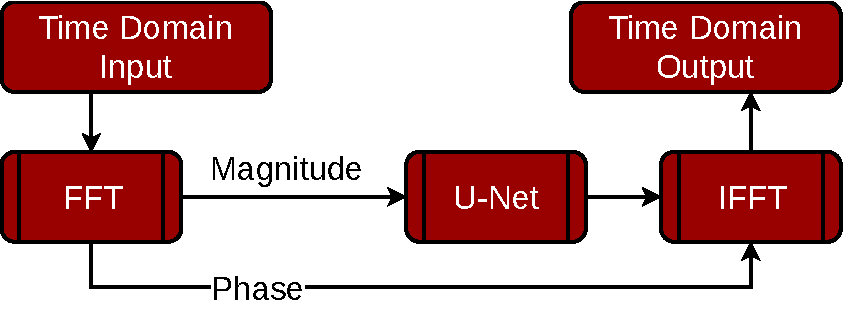
\includegraphics[width=0.5\textwidth]{systems_2}
	\caption{System Architecture of Frequency domain Network}
	\label{fig:systems}
\end{figure}
